% Klassifiziert den Dokumenten-Typ
% Doku: http://exp1.fkp.physik.tu-darmstadt.de/tuddesign/
% Farben: http://www.tu-darmstadt.de/media/medien_stabsstelle_km/services/medien_cd/das_bild_der_tu_darmstadt.pdf
%  bigchapter: Chapter haben doppelte Schriftgröße
%  linedtoc: Linien im Inhaltsverzeichnis wie bei Überschriften
%  colorbacktitle: Der Dokumenten-Titel wird mir der Accentfarbe hinterlegt
\documentclass[bigchapter,colorback,accentcolor=tud4b,linedtoc,11pt]{tudreport}

% Input Dokument hat das Encoding UTF-8
\usepackage[utf8]{inputenc}
% Wichtiges Paket für Links und verlinktes Inhaltsverzeichnis
\usepackage[ngerman]{hyperref}
% Paket für Fußnoten
\usepackage[stable]{footmisc}
% Paket für Bibliotheks-Verzeichnis, square: Verwende eckige statt runde klammern
% \usepackage[square]{natbib}
% Paket zum Plotten von Datensätzen
\usepackage{pgfplots}
% Verwende deutsche Bezeichner für Inhaltsverzeichnis, ... (ngerman = New German: neue Rechtschreibung)
\usepackage{ngerman}
% Modul für chemische Formeln
\usepackage{chemformula}
% Deutsche Zahlen (entfernt z.B. das Leerzeichen nach einem Dezimal-Komma)
\usepackage{ziffer} 

\usepackage[verbose]{placeins}


% PDF-Optionen
\hypersetup{
  pdftitle={TU Darmstadt \- Physikalisches Praktikum für Fortgeschrittene},
  pdfauthor={Manuel Kress und Sören Link},
  pdfsubject={Versuch 4.9},
  pdfview=FitH,
}
% Nummeriere formeln in Subsections einzeln
\numberwithin{equation}{subsection}
% Kleines makro zur assymetrischen Fehlerangabe
\def\tol#1#2#3{\hbox{\rule{0pt}{15pt}${#1}^{+{#2}}_{-{#3}}$}}% 

%BEGINN TITELSEITE

\title{Laserresonator}

\subtitle{Manuel Kress  \\Sören Link}

\subsubtitle{Betreuer: Patric Ackermann \hfill Versuchsdatum: 10. Februar 2014}

\author{Manuel Kress, Sören Link}

\settitlepicture{img/title.jpg}

\institution{Physikalisches Praktikum \\für Fortgeschrittene \\ Versuch 4.9}

\date{\today}

%ENDE TITELSEITE

\begin{document}
%ANFANG DOKUMENT

%Titelseite einfügen
\maketitle

%Inhaltsverzeichnis einfügen
\tableofcontents

%ANFANG INHALT

\chapter{Einleitung}

\chapter{Grundlagen}
\section{Laserprinzip}
Die Grundvorraussetzung für jeden Laser ist die Besetzungsinversion. Dazu müssen sich für zwei Energieniveaus im Lasermedium, zwischen denen ein Übergang durch Emission von Photonen erlaubt ist, im energetischeren Niveau mehr Atome befinden als im weniger energetischen. Nur wenn diese Vorraussetzung erfüllt ist, können spontan emmitierte photonen mehr Emission als Absorption anregen, da beide vorgänge proportional zur Anzahl der Atome in den zugehörigen Energieniveaus sind.

Da die Einsteinkoeffizienten für stimulierte Emission und Absorption gleich groß sind ($B_{12}=B_{21}$), ist es unmöglich, ein 2-Niveau System zum lasern anzuregen, da unabhängig von der Stärke des Pumpvorgangs und unter Vernachlässigung der spontanten Emission maximal gleichbesetzung der Niveaus 1 und 2 erreicht werden kann.

Aus diesem Grund benutzt man für Laser zumeist 3- oder 4-Niveau Systeme. Dabei werden durch den Pumpvorgang Atome vom Grundniveau $E_0$ auf ein kurzlebiges niveau $E_1$ angeregt. Dieses geht sehr schnell durch spontane Emission in den langlebigen Zustand $E_{L1}$ über. 3- und 4-Niveau Systeme unterscheiden sich dadurch, dass im 3-Niveau System der Laservorgang von $E_{L1}$ nach $E_{0}$ stattfindet, wärend im 4-Niveau System ein kurzlebiger Zustand $E_{L2}$ zwischengeschaltet ist. Dies erlaubt das Betreiben von Lasern mit einem 4-Niveau System bei bereits sehr geringer Pumpleistung, da auch bei sehr geringer Anregung bereits Besetzungsinversion zwischen den relevanten Laser-Niveaus besteht.

Beim HeNe-Laser im speziellen werden Helium-Atome durch Gasentladungen von einem Grundzustand in die Zustände $2^{9}S_{1}$ und $2^{0}S_{0}$, welche beide metastabil sind, angeregt. Die so angeregten Heliumatome geben ihre Energie durch stöße an das Neon ab, welches dadurch in den 3s bzw 2s Zustand angeregt wird. Ermöglicht wird dieser Energietransfer durch den Geringen Energieunterschied der betroffenen Helium- und Neon Energieniveaus. Der Laserforgang selbst erfolg dann beim Übergang der Neon-Atome von dem 3s zum 2p Zustand, letzterer geht dann relativ schnell durch spontane Emission in den 1s Zustand über, welcher nach Stößen mit der Wand des Verstärkermediums in den Grundzustand übergeht.

\begin{figure}[ht!]
\centering
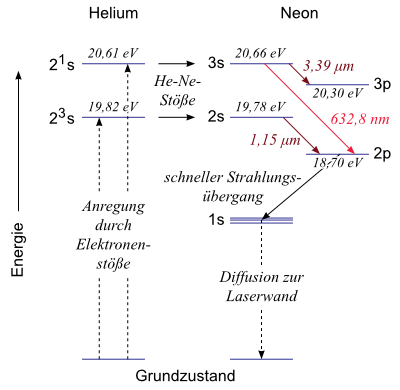
\includegraphics[width=65mm]{img/5074.png}
\caption{Energieschema eines HeNe-Lasers}
\label{HeNeLaser}
\cite{HeNeNiveaus}
\end{figure}
\section{Laserozillatoren}

\section{Resonatortheorie}

\section{Gefahren durch Laserstrahlung}

\chapter{Durchführung}
\section{Ausgangsleistung des Lasers in Abh. von der Resonatorlänge}
Zur Bestimmung der Stabilitätsgrenze des Resonaturs wurde die Ausgangsleistung für 11 Resonatorlängen aufgenommen, wobei eine Resonatorlänge innerhalb von 2 cm der errechneten Stabilitätsgrenze befand.
Die Spiegel des Laserresonators wurden dazu symmetrisch zum Verstärkermedium voneinander entfernt und die Ausgangsleistung des Resonators wurde mit dem S120C Messkopf, angeschlossen an PM100D Messgerät, aufgenommen. Anschließend wurde versucht, die aufgenommene Leistung durch Justage des Laserrohrs und der Resonatorspiegel zu optimieren.

Zu erwarten war hierbei eine annährend konstante Leistung des Lasers bis einige cm vor der Stabilitätsgrenze, mit einem kleinen Einbruch bei etwa der halben Stabilitätsgrenze.

Als Fehler für die jeweilige Spiegelposition wurden 1.5mm angenommen. Der Fehler für die aufgenommene Leistung wurde über die Fluktuation am Leistungsmessgerät abgeschätzt


\begin{center}
\begin{figure}[h]
\begin{tikzpicture}
\begin{axis}[
    title={Ausgangsleistung des Laserresonators in Abhängigkeit der Resonatorlänge},
    xlabel=Resonatorlänge in cm,
    ylabel=Ausgangsleistung in mW,
    width=0.9\textwidth,
    height= 11cm,
    xmin=20,
    xmax=92,
    grid=both,
    ymin=0,
    ymax=0.6,
    tick align=outside,
    tickpos=left,
    minor x tick num=3,
    minor y tick num=4,
    minor grid style={dotted,thin}
]
\addplot[only marks, mark=x, mark size=1pt, error bars/.cd, y dir=both, x dir=both]
table[x index={0},y index={2}, x error index ={1}, y error index={3}] {messdaten/ausgangsleistung.lvm};
\end{axis}
\end{tikzpicture}
\captionof{figure}{Ausgangsleistung des Laserresonators in Abhängigkeit der Resonatorlänge. Zu sehen ist die annährend konstante Leistugn des Resonators bis hin zu etwa 88cm und der Abfall der Leistung bei etwa der halben Stabilitätsgrenze und bei 89cm Resonatorlänge. Fehlerbalken sind eingezeichnet aber zu klein um sie zu sehen}
\end{figure}
\end{center}

\section{Strahlbreite der Grundmode in Abh. von der Resonatorlänge}

\section{Longitudinale Modensruktur in Abh. von der Resonatorlänge}

\section{Verstärkungsbandbreite des HeNe-Lasers}

\section{Beobachtung höherer transversaler Moden}

\chapter{Auswertung}
\section{Ausgangsleistung des Lasers in Abh. von der Resonatorlänge}

\section{Strahlbreite der Grundmode in Abh. von der Resonatorlänge}

\section{Longitudinale Modensruktur in Abh. von der Resonatorlänge}

\section{Verstärkungsbandbreite des HeNe-Lasers}

\section{Beobachtung höherer transversaler Moden}

\chapter{Fazit}


%ENDE INHALT

\cleardoublepage{}
% Eintrag fürs Inhaltsverzeichnis

\newpage
\begin{thebibliography}{100}
  \bibitem{mappe} Literaturmappe zum Versuch aus der physikalischen Bibliothek
  \bibitem{HeNeNiveaus} http://lp.uni-goettingen.de/get/image/5074
\end{thebibliography}

\cleardoublepage{}
% Eintrag fürs Inhaltsverzeichnis
% Abbildungsverzeichnis einfügen
\addcontentsline{toc}{chapter}{Abbildungsverzeichnis}
\listoffigures

\end{document}
